The horseshoe effect is a phenomenon that has long intrigued ecologists.  Commonly thought to be an artifact of dimensionality reduction, multiple techniques were developed to unravel this phenomenon and simplify interpretation.  Here, we provide evidence that horseshoes arise as a consequence of distance metrics that saturate - a familiar concept in other fields but new to microbial ecology.   This saturation property loses information about community dissimilarity, simply because it cannot discriminate between samples that do not share any common features. The phenomenon illuminates niche differentiation in microbial communities and indicates species turnover along environmental gradients.  Here we propose a rationale to the observed horseshoe effect from multiple dimensionality reduction techniques applied to simulations, soil samples, and samples from postmortem mice.   An intuitive-depth understanding of this phenomenon allows for the targeting of niche differentiation patterns from high-level ordination plots.
\section{Introduction}
Ecological datasets, particularly those observed in microbiome studies, are typically sparse and high-dimensional, frustrating most conventional statistical techniques.  Many numerical ecology software packages make use of distance-based statistics by calculating the distance between ecological communities, to compare various ecosystems to each other over space and time.  One of the most common exploratory analysis techniques is ordination, where the distances between the communities are embedded into a Euclidean space, and then visualized via Principal Components Analysis (\gls{pca}) \cite{numerical_ecology}.  A widely used extension of this technique, where the distance metric can be varied, is called Principal Coordinates Analysis (\gls{pcoa}) \cite{numerical_ecology}.  \par
One phenomenon that commonly occurs in datasets containing ecological gradients is the horseshoe effect or Guttman effect \cite{global_patterns}.  This phenomenon is typified by a linear gradient that appears as a curve in ordination space. The horseshoe effect, or its relative the arch effect \cite{detrended_correspondence_analysis} (where the ends of the gradient do not attract each other along the first principal coordinate as they do in the horseshoe effect), is observed using multiple types of ordinations, including Principal Components Analysis, Principal Coordinates Analysis, Non-Metric Multidimensional Scaling, Correspondence Analysis, and many others \cite{numerical_ecology}.  In 1982, the prevailing view of the horseshoe effect arose, when it was described by Gauch as a mathematical artifact that obscures the underlying ecological gradient.  Soon thereafter, Detrending Correspondence Analysis \cite{detrended_correspondence_analysis} was invented to unbend the horseshoe using reciprocal averaging. Since then, detrending has become a commonly applied practice to ordinations in ecological datasets.   Although these detrending techniques appear to provide a more intuitive visualization, they have been criticized as providing a distorted perspective of the underlying data, relying on many parameter settings that cannot be chosen in a principled way, and obscuring true underlying patterns in the data \cite{trust_dca}.\par
\begin{figure}[H]
        \centering
        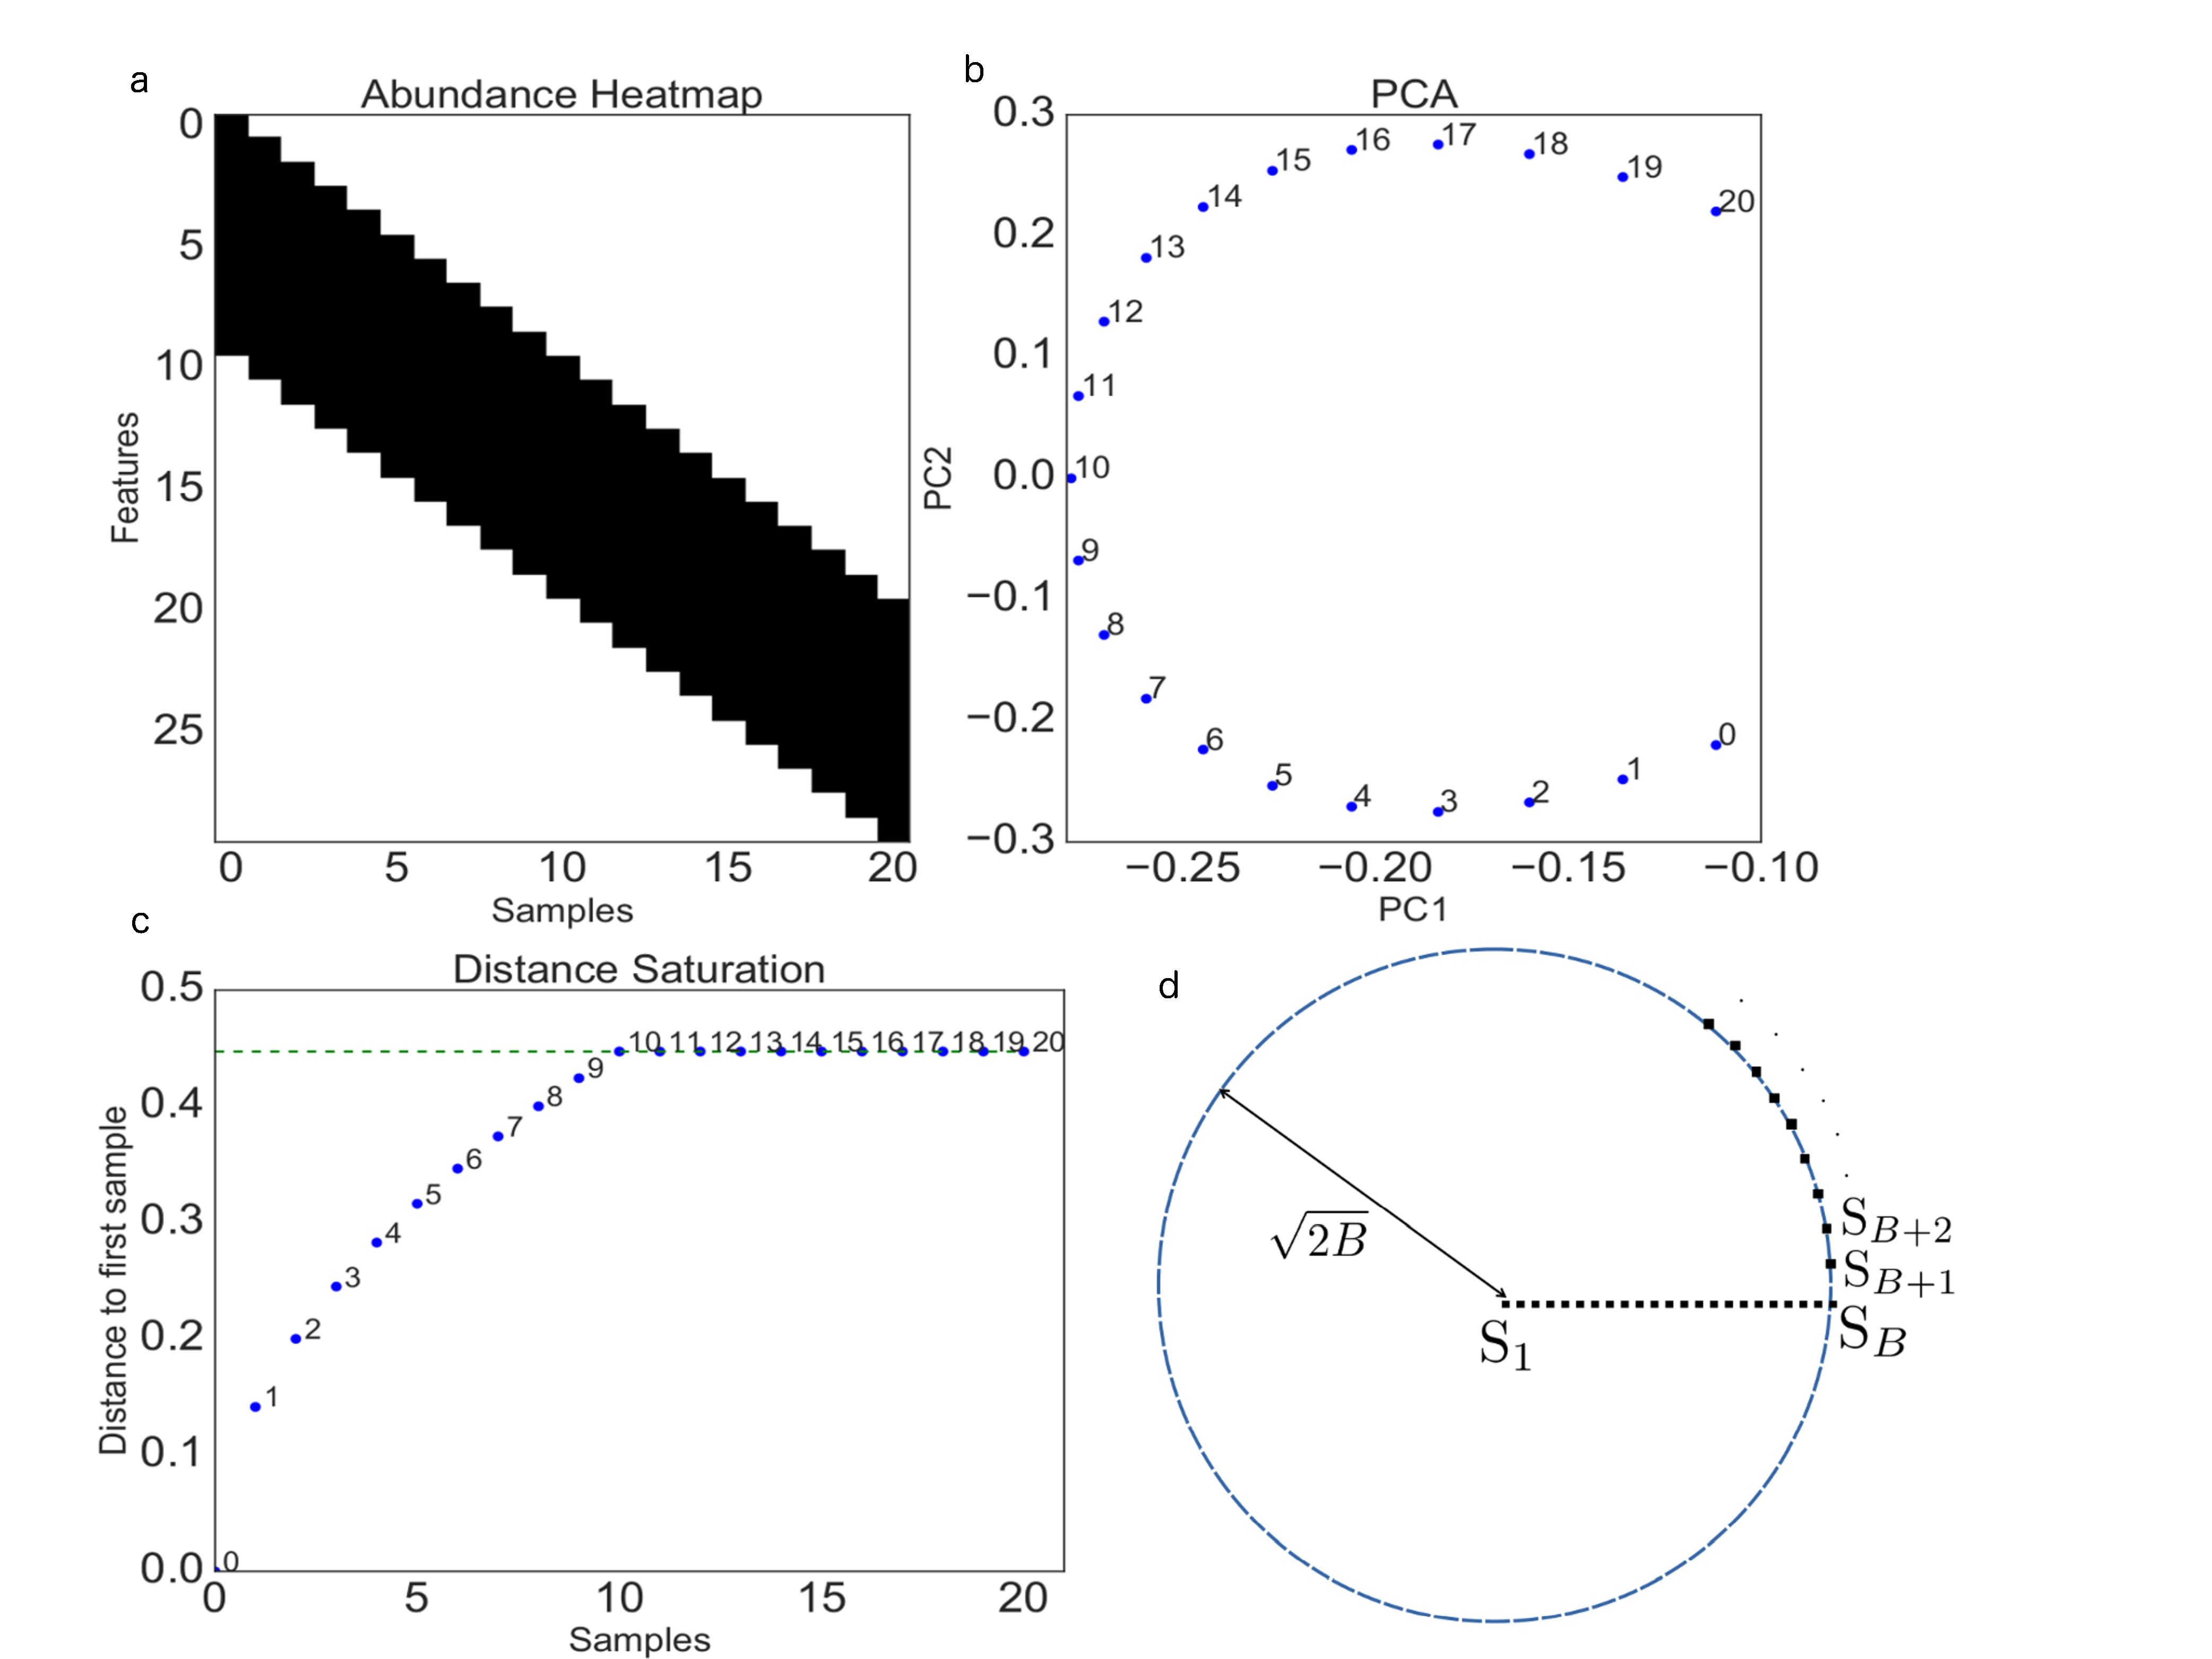
\includegraphics[width=1.1\textwidth]{ch2/Figure1.pdf}
        \caption[An explanation of the horseshoe effect arising from distance saturation.]
        {(a) A band table where the y axis encodes for individual \gls{otu}s and the x axis encodes for samples.  Blocks that are colored black have a value of 1/10 while blocks that are colored white have a value of 0.  (b) The first 2 components from a \gls{pca} of the band table, yielding the typical horseshoe shape.  (c) The Euclidean distance from the point 0 to all of the other points.  (d) An illustration of distance saturation property.\index{SanDiego6}}
        \label{figb1}
\end{figure}
From previous studies, it was shown that horseshoes can arise from band tables \cite{horseshoe_kernel} \cite{guttman_effect}.  These tables consist of highly dense, non-zero values along the diagonal of the table, and sparse values everywhere else.  This pattern can be apparent when the rows and columns are sorted in the proper order. Although the idea that band tables lead to horseshoes is not a new idea, it is commonly misunderstood how this concept applies to microbial analyses.  Here we provide some intuition behind the mathematical structure of horseshoes.\par
In Figure \ref{figb1}a, we show a simulated band table, where each vertical band is represented by a sample, and contains 10 non-zero values.  In typical microbiome datasets, these values could reflect \gls{otu} or species counts; for simplicity, here we will to refer to them as species counts, although this concept can also be generalized to multiple data types, such as gene counts, metabolite abundances.  Each sample in the table is shifted by 1 row, creating the band effect.  When \gls{pca} is applied directly to this table, the first 2 eigenvectors yield a horseshoe pattern (Figure \ref{figb1}b).  Here, the band table is parameterized with a band size of 10, since each sample has exactly 10 non-zero values.  \par
For close local points, the Euclidean distance grows linearly along the gradient (Figure \ref{figb1}c).  However, after a certain point, the distance completely saturates. This property has been previously noted with Euclidean distance \cite{detrended_correspondence_analysis}.  The overlap between the first sample in the band table, and sample 10 and beyond disappears, and the distance between these samples is maximized. This can yield unintuitive properties, sample 10 could be less dissimilar than sample 1 compared to sample 20.  For instance, sample 10 could represent a medium pH environment, sample 1 could represent an acidic low pH environment and sample 20 could represent a high pHbasic environment. Sample 1 is expected to a substantially more different microbial community to Sample 20 than Sample 10.  The acidophiles that found in Sample 1 are typically not found in basic environments. Sample 20 is expected to be more different to sample 1 than sample 10, since contains very different microbes that thrive in high pH environments.  But as far as Euclidean distance is concerned, sample 10 is just as dissimilar to sample 1 as sample 20, just because there are no common bacteria shared between these samples.  It is apparent that the saturation property of Euclidean distance does not capture all of the information about community dissimilarity along a gradient, simply because it cannot discriminate between samples that do not share any common features.  Once the distance is saturated, all samples that do not overlap lie within a ball of radius B where B is the band sizelie within a ball of radius where B is the band size and the first point is the center of the ball as shown in Figure \ref{figb1}d.\par
This saturation property has been suggested to give rise to horseshoes in previous studies in other fields \cite{horseshoe_kernel}, and is an unintuitive property that can confound ecological interpretations if not understood properly.  This property also restricts the possible trajectories of samples in the feature space, and gradients cannot be represented by linear trajectories in the real space (Supplemental proof 1). This means that communities in the original high dimensional space do not arrange into linear trajectories in the first place, and when projected to lower dimensions do not fall into linear trajectories.  These trajectories are what we refer to as horseshoes.  The horseshoe phenomenon is analogous to the familiar concept of saturation in molecular evolution, where two randomly evolving sequences saturate at 75\% DNA sequence identity (assuming equal nucleotide frequencies), even if infinite time has elapsed \cite{dna_saturation}. Consequently, distances that reflect a higher degree of molecular change need to be corrected for multiple substitutions in order to recover the molecular clock-like behavior obtained when comparing more similar sequences. This is why corrections according to models such as Jukes-Cantor or the Kimura 2-parameter model are required to obtain distances for reconstructing better phylogenetic trees. Analogous distance corrections are needed in microbial ecology for reconstructing better relationships among microbial communities \cite{evolutionary_distances}.\par
It is important to note that horseshoes do not only arise from \gls{pca}, but also arise in \gls{pcoa} with a variety of distance metrics.  Arch effects have plagued every multidimensional reduction technique we have applied to a wide range of microbial ecology datasets \cite{microbial_patterns}. In the following case studies, we'll show that these distance metrics also have the saturation property.  In addition, if a distance doesn't have this saturation property, there won't be an observed horseshoe artifact (Figure S1).\par
\section*{Case Study 1 - 88 Soils}
In this study, 88 soil samples were obtained from multiple locations across the United States having varying levels of pH \cite{soil_pyro}.  The V4 region of the 16S rRNA gene (16S) within each organism was amplified and sequenced using 454 pyrosequencing to obtain relative abundances of microbial taxa.  A matrix representing abundance values for each taxonomic unit per soil sample was used as input in correspondence analysis (\gls{ca}) \cite{correspondence_analysis}. The resulting ordination showed clear separation of the communities based on pH (Figure \ref{figb2}a), which led to the same conclusion that pH is a major driving factor in soil biogeography, i.e. pH has major impacts on the distribution of bacterial taxonomic units in soil \cite{soil_pyro}.  The \gls{ca} analysis in Figure \ref{figb2}a also shows the classic horseshoe shape.   Here we revisited this study, to better understand the horseshoe shape behind this dataset.\par
To test the effect of another commonly used distance metric on the sample distribution, we analyzed the same soil dataset applying Chi Squared distance (Figure \ref{figb2}b). Similar to what was observed with Euclidean distance, which was applied in the simulation, the Chi Squared distance increased sharply at pH 3 and 4, but began to saturate at pH of 5.  Also the band table similar to what we have observed in Figure \ref{figb2}a can be obtained when sorting.  Also, when the the \gls{otu} table was sorted by sample pH and the mean pH of the samples that the \gls{otu}s were observed in mean pH of the \gls{otu}s (Equation 12), the same band table pattern appeared as we show in Figure \ref{figb2}a.  While the diagonal isn't completely dense, there are more non-zero values compared to the corners of the heatmap. In line with the findings from the original study, this pattern is likely representative of niche differentiation of \gls{otu}s with respect to pH. The organisms that thrive in low pH environments tend not to exist in high pH environments and vice versa.  Low pH and high pH samples are shown in Figure \ref{figb2}c to have few overlapping species, a pattern not observed in the original study as membership was evaluated at coarser levels of taxonomic resolution\cite{soil_pyro}.\par
\begin{figure}[H]
        \centering
        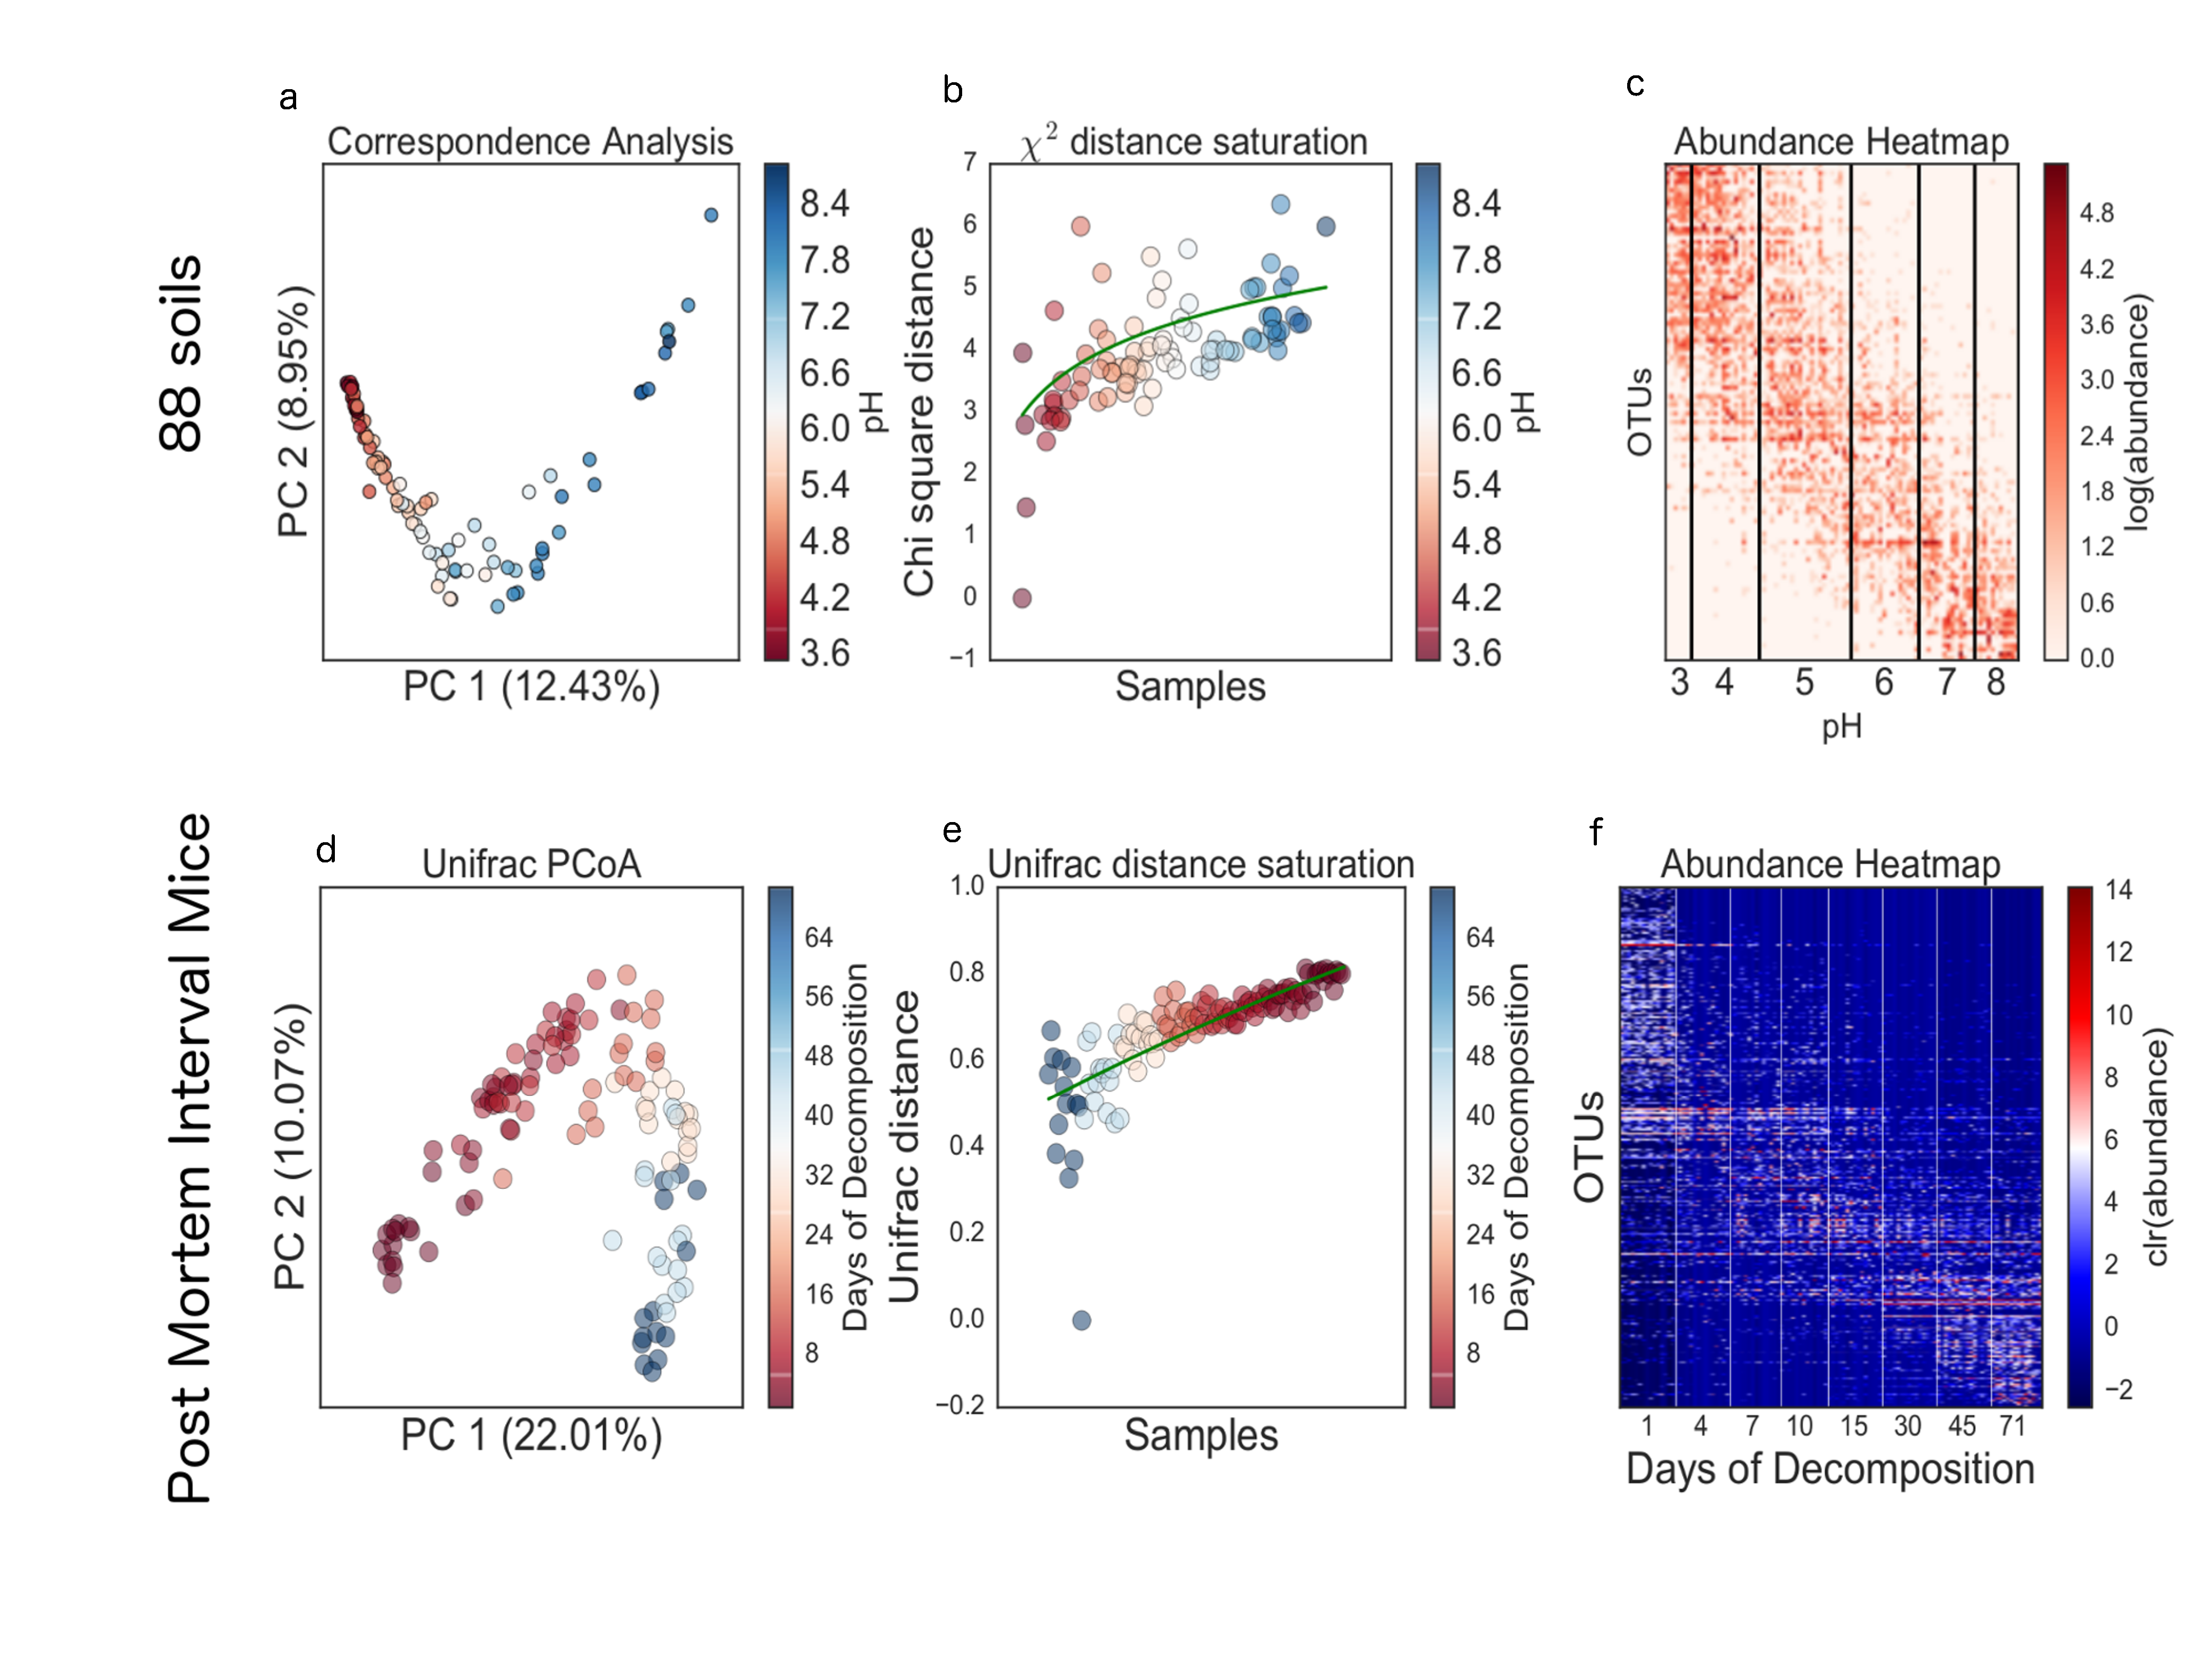
\includegraphics[width=1\textwidth]{ch2/Figure2.pdf}
        \caption[Two case studies show casing how horseshoes can appear in the context of
          soil microbial communities and post-mortem microbial communities.]
        {(a) Correspondence analysis of 88 soils.  (b) Distance saturation of chi-squared metric, plotting the chi squared distance of the first sample versus all of the other samples. (c) Heatmap of log transformed \gls{otu} counts from the 88 soils with the samples sorted by pH and the \gls{otu}s sorted by mean pH.  (d) Principal Coordinates Analysis of unweighted UniFrac distance.  (e) UniFrac distance of a samples from the last time point versus all of the samples. (f) Heatmap of centred log ratio transformed (Equation 2) \gls{otu} counts sorted by harvest days.\index{SanDiego8}}
        \label{figb2}
\end{figure}
\section*{Case Study 2 - Post Mortem Mice Study}
In this study, 120 mice were sacrificed and allowed to decompose on soil. Mice were destructively sampled over approximately 8 weeks\cite{mammalian_corpse}. 16S sequencing libraries were generated from total DNA extracted from swabs of the skin on the head, and relative abundance values were calculated for each bacterial \gls{otu}. A relative abundance matrix was generated for each library and used as input in \gls{pca}. This analysis generated a clear horseshoe (Figure \ref{figb2}d) using unweighted UniFrac distance \cite{soil_pyro}, with a gradient with respect to the time since death, possibly reflecting a changing skin microbiome during decomposition of the mouse carcass. When the samples were sorted by time since death using a similar strategy as noted above, a band table emerges (Figure \ref{figb2}f). Also, the unweighted UniFrac distance analysis appears to have the same saturation property as observed previously with Euclidean distance and Chi-squared distance.  It is important to note that highest possible UniFrac distance is 1, suggesting that this distance metric can also be saturated.  In Figure \ref{figb2}e, while the distance hasn't completely saturated, these distances are quickly approaching the theoretical maximal UniFrac distance. \par
The striking changes in microbial communities during decomposition are associated with dramatic environmental biochemical changes, including increased pH, ammonia, and total nitrogen, all measured in soil beneath the mice. Correspondingly, microbial communities are predicted to increase in gene abundance of important nitrogen cycling pathways such as amino acid degradation (e.g. glutamate dehydrogenase, lysine decarboxylase, ornithine decarboxylase) and nitrate reduction (e.g. nitrate and nitrite reductase). Bacterial taxa in the families Chromatiaceae (\gls{otu} 46026, 4482362) and Rhizobiaceae (\gls{otu} 4301099) are involved in nitrogen metabolism and become abundant as mouse bodies progress through the stages of decomposition (e.g. Fresh, Active Decay, Advanced Decay).  As shown in Figure S1, all of these \gls{otu}s peak at specific timepoints. The two Chromatiaceae \gls{otu}s peak during Active Decay (bloating and purge of fluids) at 15 days of decomposition. The Rhizobiaceae \gls{otu} peaks during Advanced Decay (sinking and sagging flesh) at 30 days of decomposition and when pH, ammonia, and total nitrogen were measured at their highest levels \cite{mammalian_corpse}.\par
To further validate if saturation leads to horseshoes, a new distance metric \gls{embad} (Earth Mover Band Aware Distance) was engineered to be non-saturating as a proof of concept (Supplemental Methods).  This distance metric uses prior knowledge about the ordering of the band table, and is determined by calculating the flow between two samples. As shown in Figure S1a, sample 1 and sample 2 each have 4 species proportions.  To calculate the distance between sample 1 and sample 2, the probability mass of species 1 and species 2 needs to be shuffled over to species 3 and species 4.  This concept is analogous to computing maximum flow along a pipe, and can be calculated using Earth Mover's distance \cite{emd}\cite{unifrac_emd}\cite{unifrac}.\par
For the 88 soils (Figure S1b), the \gls{embad} was applied to the pH sorted table. Therefore, even if two samples are not overlapping, samples closer together will have a smaller distance than samples further apart in the gradient.  This is because the distance is defined to be not saturating and explicitly accounts for the pH gradient.  The same strategy was employed for the postmortem interval mice (Figure S1c), sorting the table by decomposition days. The \gls{pcoa} plots resulting from these applications of \gls{embad} suggest that a non-saturating distance metric could remove the horseshoe effect from lower dimensional projections of these abundances.  This provides further evidence that this saturation property could explain the the horseshoe phenomenon.\par
For the 88 soils study a \gls{permanova} test investigating the difference between soils with a pH less than 3, and soils with a pH greater than 8.  With the \gls{embad} distance metric the \gls{permanova} gave a pseudo F-statistic of 650.5 and a p-value of 0.0003, which has a much larger effect size compared to the original Chi-squared distance metric with a pseudo F-statistic of 3.8 and a p-value of 0.0004 with 9999 permutations.  A similar trend was observed in the post mortem interval mice study when testing the first decomposition day to the last decomposition day using \gls{permanova}.  The \gls{embad} distance metric had a pseudo F-statistic of 439.8 and a p-value of 0.0001 with 9999 permutations, which has a larger effect size than the Unifrac distance metric, which had a pseudo F-statistic of 25.5 and a p-value of 0.0001. This method is relieved from misinterpretations of data due to horseshoes and arches and facilitates the interpretation of taxonomic units along biologically significant gradients that reflect the selective pressure of these factors on the distribution of microbes.  \par
In light of the benefits of engineering a non-saturating distance metric, the \gls{embad} distance metric requires the gradient to known a priori.  Generalizing this approach in the absence of known gradients is a difficult problem would require an exhaustive using known algorithms.  Specifically, this problem falls under the category of NP-hard problems (Supplemental Proof 2).  In the 88 soils study and the post mortem mice study, we were fortunate to be able to infer the underlying band table with known metadata.  \par
The band patterns we observe here are probably very common in ecology studies investigating species distribution patterns across spatial or temporal gradients. The pattern confirms microbial ecological fundamentals, i.e. bacteria have acquired unique adaptations to the environment and occupy either a broad range or very specific niches. In our case studies of the 88 soils - and the postmortem mice we confirmed that by using a band table pattern analysis approach, bacterial species show different adaptations to pH and bacterial diversity changes over time during decomposition of mice carcasses. The band pattern approach we apply here represents an additional method to visualize differences between microbial communities.\par
Based on our observations here, the horseshoe effect appears in dimensionality reduction techniques due to the saturation property of distance metrics.  While we have only tested a few distance metrics, it is suspected that a vast majority of these distance metrics exhibit the same property, which would also explain why horseshoes are encountered so frequently across many different fields. The saturation property has also been observed in multiple other fields, and other studies from different disciplines have come to similar conclusions \cite{horseshoe_kernel}. In addition, multiple techniques such as self organizing maps \cite{self_organizing_maps} and local linear embedding \cite{local_linear_embedding} attempt to avoid this saturation phenomenon by focusing on distances of nearby points.\par
In spite of the saturation property of distance metrics, identifying horseshoes is still highly useful for identifying patterns concerning niche differentiation.   Properly understanding this phenomenon will motivate the use and development of algorithms such as biclustering \cite{biclustering} to uncover underlying band patterns.  These insights will in effect allow us to identify microbial niches along different environmental conditions.\par
\section{Materials and Methods}
All analyses can be found below on github \\
\url{https://github.com/knightlab-analyses/horseshoe-analyses}.
The mean gradient used for the 2 case studies was calculated as follows.
\begin{equation}
        \overline{g}_{x}=\sum_{i=1}^{N}g_{i}\frac{x_{i}}{\sum_{j=1}^{D}x_{j}}
\end{equation}
Where $x_{i}$ is the proportion of \gls{otu} \textit{x} in sample \textit{i} , $\overline{g}_{x}$ is the mean gradient of \gls{otu} \textit{x}, and $g_{i}$  is the sample gradient at sample i. This calculation can be found in the gneiss package under the function \textbf{mean\_niche\_estimator}. The function used to sort the tables in Figure \ref{figaS1}c used \textbf{niche\_sort}. In the 88 soils study, the table was sorted by sample pH and the mean pH of the samples that the organisms were observed in. In the post mortem mice study, the table was sorted by the days of decomposition and the mean day of the samples of that the organisms were observed in.\par
The heatmap in Figure \ref{figaS2}f and the abundances in Figure S2 were normalized using the centre log ratio transformation given by the following equation.
\begin{equation}
        \gls{clr}(x)=\left [ ln\frac{x_{1}}{g(x)},...,ln\frac{x_{D}}{g(x)} \right ]=lnx-\overline{lnx}
\end{equation}
Where $g(x)=\sqrt[n]{\prod_{i=0}^{n}x_{i}}$ is the geometric mean and $\overline{lnx}=lng(x)=\frac{1}{n}\sum_{i=0}^{n}lnx$ is the average of the log transformed values.  A pseudocount of 1 is added to all of the counts to prevent logarithms of zero occurring. \par
Analyses were performed using Scipy, Numpy, Matplotlib, Seaborn, Scikit-bio and Gneiss.
\section{Acknowledgements}
We thank Noah Fierer for his input on the analysis of the 88 soil samples and Dan Knights for discussion on the \gls{embad} metric. We also acknowledge Amnon Amir and Tomasz Kosciolek for their insights into the horseshoe effect. Finally, we thank Susan Holmes for her insights on previous work understanding the horseshoe effect.

J.T.M. was funded by NSF GRFP DGE-1144086. J.L.M. and R.K. were funded by the Office of Justice Programs National Institute of Justice (award NIJ-2011-DN-BX-K533).
